\chapter{Projektafgrænsning (JS)}

Grundet begrænset tid og ressourcer er det nødvendigt fra start at sætte nogle begrænsninger til hvilke dele af systemet der ønskes realiseret, som det ligeledes har været nødvendigt under forløbet at skære ned på hvad vi har ønsket realiseret. 

X10 opererer normalt på 230 Vac el-nettet, men da vi ikke har autorisation til at arbejde med 230 V og af sikkerhedsmæssige årsager foregår realiseringen ved 18 V 50 Hz. Dette ændrer ikke på funktionaliteten eller virkemåden af systemet. 

Lyddetektionen og magnetlåse er desværre ikke nået realiseret som ønsket.
For lyddetektionen er der er i stedet lavet med en knap der giver et højt signal som skal imitere at lyd er detekteret. Se figur \ref{fig:BABY_ALARM}. 
Der er ikke lavet nogen alternativ løsning til magnetlås.

\begin{figure}[htbp]
  \centering
    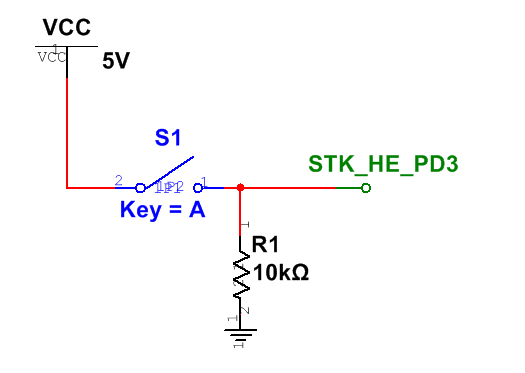
\includegraphics[width=0.5\textwidth]{billeder/BABY_SWITCH}
    \caption{Diagram over knap for lyddetektion}
    \label{fig:BABY_ALARM}
\end{figure}

